The primary objectives of the motion model are global synchronization,
\emph{Web availability} and simplicity for Web developers. Global
synchronization implies media synchronization across the Internet. Web
availability means that no additional assumptions can be introduced for media
synchronization. If a Web browser is able to load an online Web page, it
should also be able to synchronize correctly. The model proposed for this can
be outlined in three simple steps:

\begin{itemize}
\item{Media clock and media controls are encapsulated in one concept, and
represented as a stateful resource. This chapter uses the term \emph{motion}\footnote{\emph{motion} as in \emph{motion pictures}. \emph{Moving through media} still remains a good way to conceptualize media experiences, not least as media experiences become virtual and immersive.
} for this
concept.} 
\item{A \emph{motion} is an online resource, implying that it is hosted by a
server and identifiable by URLs.}
\item{\emph{Media components}\footnote{\emph{media component:} anything from a simple $<div>$ tag with text, to a highly sophisticated media player or multimedia framework.
} synchronize themselves relative to online motions.}
\end{itemize}

According to the model, media synchronization should be a consequence of
connecting multiple media components to the same online motion. This way, rich
synchronized multi-device presentation may be crafted by connecting relevant
media components to the same online motion. 

\begin{figure}[h]
%\sidecaption
\centering
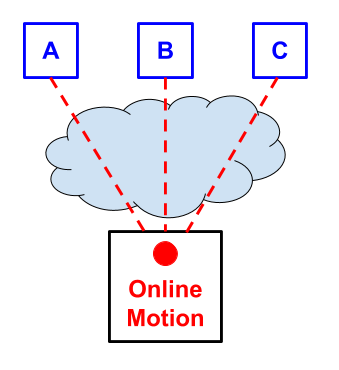
\includegraphics[scale=.4]{fig/motion-model.png}
\caption{Media components on three different devices (A,B,C), all connected to an online motion
(red circle). Media control requests (e.g. pause/resume) target the online motion and are transmitted across the Internet (light blue cloud). The corresponding state change is
communicated back to all connected media components. Each media component
adjusts its behaviour independently.}
\label{fig:model}
\end{figure}

Importantly, the practicality of the motion model depends on Web developers
being shielded from the complexities of distributed synchronization. This is
achieved by having a \emph{timing object} locally in the Web browser. The
timing object acts as an intermediary between media components and online
motions, as illustrated by Fig.~\ref{fig:model-2}. This way, the challenge of
media synchronization is divided in two parts.

\begin{itemize}
\item{\emph{motion synchronization}: timing object precisely synchronized with online motion (Internet problem).}
\item{\emph{component synchronization}: media component precisely synchronized with timing objects (local problem).} 
\end{itemize}


\begin{figure}[h]
%\sidecaption
\centering
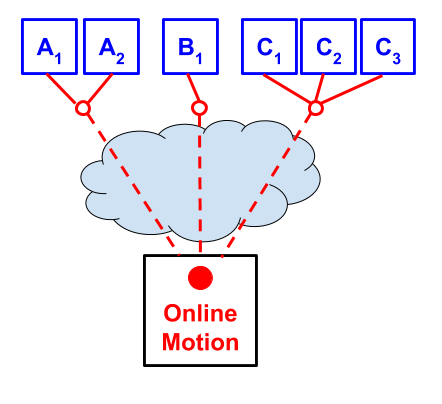
\includegraphics[scale=.4]{fig/motion-model-2.png}
\caption{Timing objects (red unfilled circles) mediate access to online motion. Timing objects may be shared by independent mediacomponents within the same browing context.}
\label{fig:model-2}
\end{figure}

\emph{Motion synchronization} ensures that timing objects connected to the
same online motion are kept precisely synchronized. The logic required for
motion synchronization could be supported by Web browsers natively (if
standardized), or imported into Web pages as a third party JavaScript
library. Motion synchronization is outlined in Sect.~\ref{sec:motionsync}.

\emph{Component synchronization} implies that a media component continuously
strives to synchronize its activity relative to a timing object. As such,
component synchronization is a local problem. Media components always
interface with timing objects through a well defined \emph{API} (see
Sect.~\ref{sec:motionapi}). Examples of component synchronization are provided in Sect.~\ref{sec:avsync} and Sect.
~\ref{sec:sequencer}.

